\section{Numerical Discretization Error vs. Turbulence Modeling Uncertainty}\label{sec:num_vs_turb_error}

Solving continuous equations on a discrete domain creates numerical discretization error.
In RANS CFD simulations, the continuous RANS equations that define fluid flow are solved on a discrete domain known as the mesh or grid.
Numerical discretization error can be reduced by increasing the number of discrete points in the domain.
As the discretization increases and the grid spacing tends towards $0$, the numerical error approaches $0$ as well. 
This is the basis for the "Grid Convergence Study" method for quantification of numerical discretization error \cite{american_society_of_mechanical_engineers_standard_2009}.
Details of the methodology are reproduced here for clarity.

The methodology requires the use of a family of grids that are sequentially coarser but are generated using the same grid generation parameters.
This is most easily done with structured meshes where a very dense grid, which would result in minimal discretization error, is first generated.
Then each successive coarser grid level removes every other grid line in each direction.
In 2D and 3D computations, this results in the number of grid point reducing by a factor of 4 and 8 respectively, at each grid level.
It results in grids that are uniformly refined which isolates the effect of the discretization on the simulations. 

Three grids of successive refinement are required to calculate all the numerical error metrics. 
First, a representative grid size for the $i$-th grid is defined as
\begin{equation} \label{equ:grid_h}
    h_i = \left ( \frac{1}{N_i}\right )^A
\end{equation}
where $N_i$ refers to the number of degrees of freedom in the $i$th grid and $A=1/2$ for 2-D simulations and $A = 1/3$ for 3-D simulations.
SU2 uses node-centered numerics, so $N_i$ refers to the number of nodes in the grid.
The grids are ordered such that $i=1$ refers to the finest grid (most number of nodes) and $i=3$ refers to the coarsest grid.
Correspondingly, a smaller value of $h$ indicates a finer mesh with more nodes. 
Next, grid ratios are defined as 
\begin{equation}
    r_{21} = \frac{h_2}{h_1},~r_{32} = \frac{h_3}{h_2},
\end{equation}
and solution differences are defined as
\begin{equation}
    \epsilon_{21} = \phi_2 - \phi_1,~\epsilon_{32} = \phi_3 - \phi_2,
\end{equation}
where $\phi_i$ is the solution on the $i$-th grid.
Often for aerodynamics-related problems $\phi$ represents a force or moment coefficient such as $C_L$ or $C_m$.

These quantities can be used to compute the observed order of convergence, $p$, by solving the following equations using a fixed point iteration:
\begin{align}
    p & = \frac{1}{\ln{\left ( r_{21} \right )}} \left ( \ln{\left \vert \frac{\epsilon_{32}}{\epsilon_{21}} \right \vert } + q(p) \right )
    \\
    q(p) & = \ln{ \left ( \frac{r_{21}^{p} - s }{r_{32}^{p} - s}\right )}
    \\
    s & = 1\times sign \left ( \frac{\epsilon_{32}}{\epsilon_{21}}\right ).
\end{align}
The order of convergence should be close to the order of the numerical method used to solve the simulations. 
2nd order numerical methods are used for all of the RANS calculations made using SU2 and so we expect the observed order to be close to $2$.

Using the grid ratios and the apparent order of convergence, the infinite grid solution can be extrapolated as,
\begin{equation}
    \phi_{ext}^{21} = \frac{r_{21}^p\phi_1 - \phi_2}{r_{21}^p - 1}.
\end{equation}

The approximate relative fine-grid error: 
\begin{equation}
    e_a^{21} = \left \vert \frac{\phi_1 - \phi_2}{\phi_1} \right \vert,
\end{equation}
can be used to calculate the fine-grid convergence index:
\begin{equation}
    GCI_{fine}^{21} = \frac{1.25e_a^{21}}{r^p_{21}-1}.
\end{equation}
Here $1.25$ is an empirically recommended Factor of Safety based on hundreds of CFD case studies \cite{roache1998verification}.
Furthermore, the GCI can be used to express the $95\%$ confidence interval on the fine grid solution. 
The solution can be expressed as
\begin{equation} \label{equ:num_error_bars}
    \phi \approx \phi_1 \pm \left( GCI_{fine}^{21} \right)\left \vert \phi_1 \right \vert 
\end{equation}

Armed with these metrics to quantify the numerical discretization error in the CFD simulations, comparisons to the uncertainty introduced by turbulence models can be made. 
The eigenspace perturbation methodology discussed in Section \ref{sec:equips_rans_uq} only estimates uncertainties introduced by turbulence models.
The RANS CFD simulations required to quantify the uncertainties are run on grids that introduce some degree of discretization error.
The following sections explore the relationship and the relative magnitudes of the two quantities.

\subsection{NACA0012 Airfoil} \label{sec:num_err_naca0012}

The same NACA0012 case presented in Section \ref{sec:equips_naca0012} is used here. 
This case is used in the 5th and 6th Drag Prediction Workshops as a verification study \cite{levy2013summary,roy2017summary}.
The grids that were used for those verification studies are used here, details for which are shown in Table \ref{tab:naca0012_meshes}.

\begin{table}
    \renewcommand{\arraystretch}{1.2}
    \centering
    \begin{tabular}{ c|c|c|c|c } 
%  \hline
         Mesh Level & Nodes & Surface Nodes & Wall spacing & Approx. $y^+$  \\ 
         \hline
         L1 & $14,687,744$ & $4,097$ & $1.0\times10^{-7}~m$ & 0.025\\
         L2 & $3,673,856$ & $2049$ & $2.0\times10^-7~m$ & 0.05\\
         L3 & $919,424$ & $1,025$ & $4.0\times10^{-7}~m$ & 0.1\\
         L4 & $230,336$ & $513$ & $8.0\times10^{-7}~m$ & 0.2\\
         L5 & $57,824$ & $257$ & $1.6\times10^{-6}~m$ & 0.4\\
         L6 & $14,576$ & $129$ & $3.2\times10^{-6}~m$ & 0.8\\
         L7 & $3,584$ & $65$ & $6.4\times10^{-6}~m$ & 1.6\\
        
    \end{tabular}
    \caption{Details of the grid family used to perform numerical discretization error quantification for the NACA0012 case.}
    \label{tab:naca0012_meshes}
\end{table}

To be consisted with the results form the eigenspace perturbation methodology, the SST turbulence model is used for these simulations. 
The grid convergence trends for $C_L$ and $C_D$ are shown in Figure \ref{fig:naca0012_mesh_convergence}.
The $x$-axis for the figures is the representative mesh size $h$ (Equation \ref{equ:grid_h}). 
Going from right to left on the $x$-axis corresponds to increasing grid refinement, from the L7 mesh to the L1 mesh. 
As the grid refinement increases the coefficients converge towards the infinite grid solution.

Ideally, to compare the numerical discretization error and the turbulence modeling uncertainty, the finest three meshes woul

\begin{figure}
\center
\subfigure%[\label{subfig:naca0012_tmr_CL} Coefficient of pressure variation over the upper surface of the airfoil at $\alpha=10^{\circ}$]
  {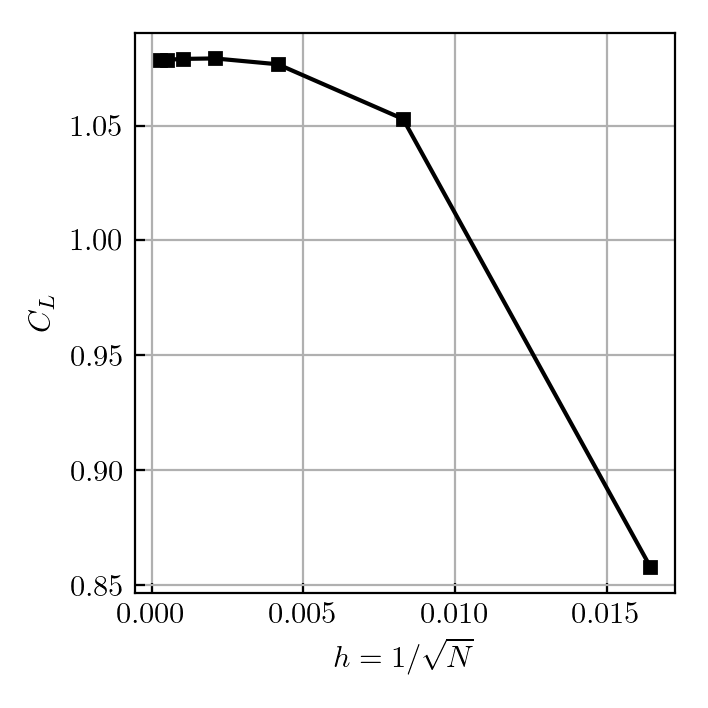
\includegraphics[width=0.48\textwidth]{code/image_gen/naca0012/images/naca0012_CL_tmr_mesh_convergence.png}}
\subfigure%[\label{subfig:naca0012_tmr_CD }Coefficient of pressure variation over the upper surface of the airfoil at $\alpha=15^{\circ}$]
  {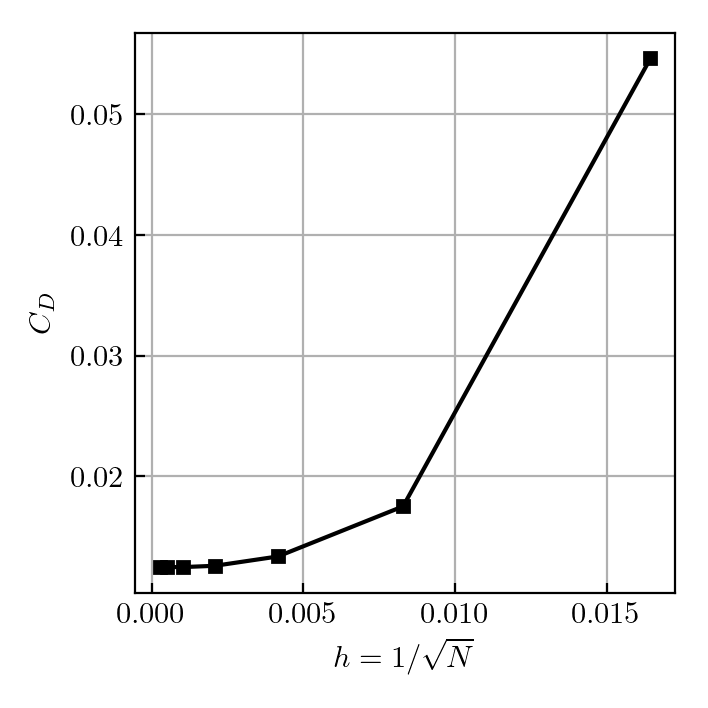
\includegraphics[width=0.48\textwidth]{code/image_gen/naca0012/images/naca0012_CD_tmr_mesh_convergence.png}}
\caption{Effects of grid refinement on $C_L$ and $C_D$ predictions at $\alpha = 10^\circ$ for the NACA0012 airfoil.}\label{fig:naca0012_mesh_convergence}
\end{figure}

For this case the $GCI_{fine}^{43} = 5.0 \times 10^{-5}$ which represents a $95\%$ confidence interval of $1$ drag count ($10^-4$). 
This is a suitably low numerical discretization error that would not adversely affect the RANS CFD simulations. 
The finer meshes, L2 and L1, are computationally expensive to perform simulations on.
So to compare the numerical discretization error and the uncertainties predicted by the eigenspace perturbation methodology, the L3, L4, and L5 meshes are used. 
The L6 mesh, which has significant numerical error as evidenced by its under-prediction of $C_L$ and over-prediction of $C_D$, is also explored to see how the RANS UQ methodology handles insufficient discretization that might not capture relevant flow features. 

The RANS UQ methodology is applied to each of the meshes in question, L3-L6.
The same $\alpha$ sweep that was used in Section \ref{sec:equips_naca0012}, $0^\circ \leq \alpha \leq 20^\circ$, is used for these simulations. 
The $C_L$ vs. $\alpha$ sweep for all the meshes are shown in Figure \ref{fig:naca0012_mesh_sweeps}. 
Figure \ref{subfig:naca0012_CL_tmr_rans_uq} shows the results of the individual baseline simulations using the different mesh levels. 
As the mesh refinement is increased, going from L6 to L3, the simulation results tend to agree more with the experimental data. 
This is expected as the numerical discretization error in the simulations is being reduced by increasing the number of grid points in the mesh. 
Figure \ref{subfig:naca0012_CL_tmr_rans_uq} overlays the turbulence modeling uncertainty estimates from the EQUiPS module onto the $\alpha$ sweep results.
The color of the uncertainty area corresponds to the mesh level represented.
It is hard to distinguish between the uncertainty areas from the L3-L5 meshes because all of these uncertainty areas are almost exactly coincident.
The notable exception is the uncertainty estimate for the L6 mesh in blue. 
These two observations indicate that while a minimum grid refinement that captures the relevant flow features is required, further grid refinement does not significantly impact the uncertainty estimate predicted by the eigenspace perturbation methodology.
This is a significant conclusion as it means that uncertainty quantification can be performed using coarser meshes that reduce the computational cost of performing the 6 simulations required to engender the uncertainty estimate. 

\begin{figure}
\center
\subfigure[\label{subfig:naca0012_CL_tmr} $C_L$ vs. $\alpha$ sweeps meshes of varying refinement.]
  {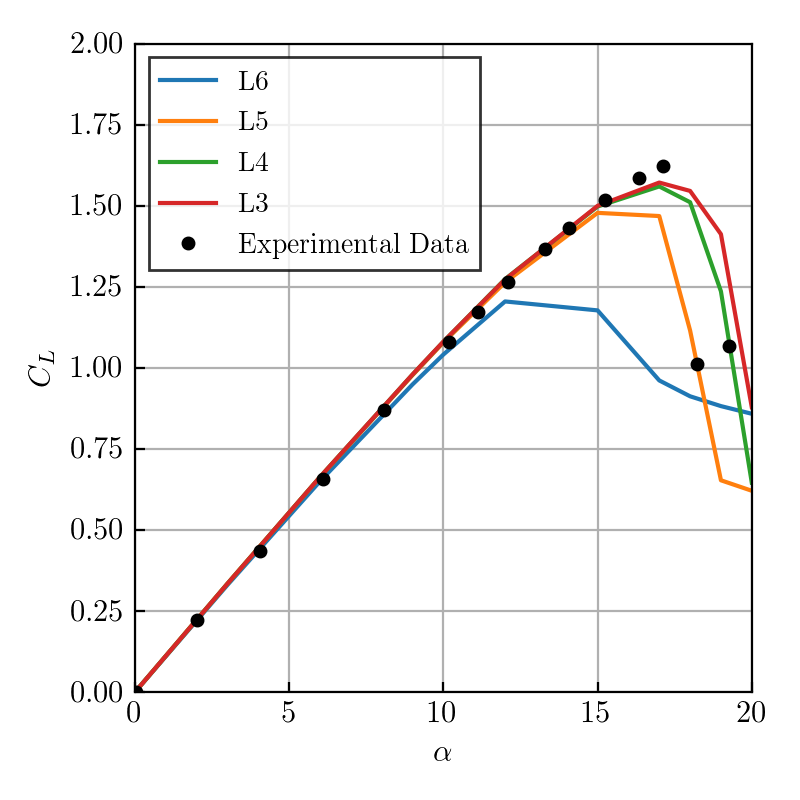
\includegraphics[width=0.48\textwidth]{code/image_gen/naca0012/images/naca0012_cl_vs_alpha_tmr_meshes.png}}
\subfigure[\label{subfig:naca0012_CL_tmr_rans_uq} $C_L$ vs. $\alpha$ sweeps with the corresponding turbulence modeling uncertainty areas overlaid on the plot]
  {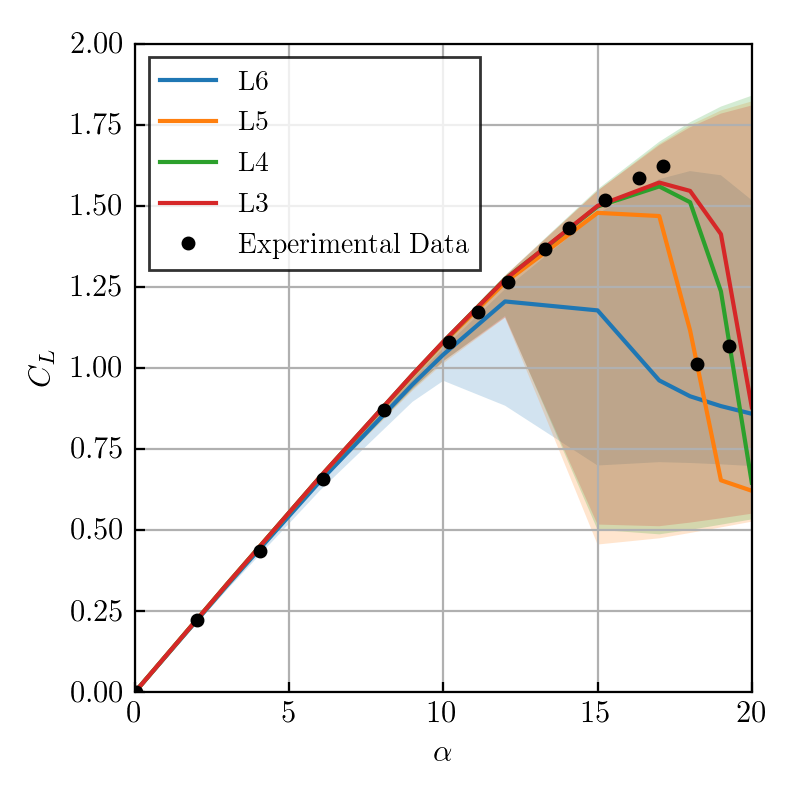
\includegraphics[width=0.48\textwidth]{code/image_gen/naca0012/images/naca0012_cl_vs_alpha_tmr_meshes_uq.png}}
\caption{Results of using the eigenspace perturbation methodology to estimate the turbulence modeling uncertainties in $C_L$ predictions at a range of $\alpha$ values. }\label{fig:naca0012_mesh_sweeps}
\end{figure}

Lastly, the relative magnitude of the numerical error to the turbulence modeling uncertainty is explored in Figure \ref{fig:naca0012_num+turb_uq}. 
The L3-L5 meshes are used to compute the numerical error metrics. 
The error bars on the simulation data points represent the $95\%$ confidence interval on the numerical discretization error as defined by Equation \ref{equ:num_error_bars}.
The blue shaded area is the turbulence uncertainty estimate. 
For most of the points, the discretization error bars are too small to be visible at this scale.
The turbulence uncertainty is greater than the discretization error bars for most of the simulations, even those at lower angles of attack. 
But care must be taken when talking about the simulations at higher angles of attack. 
The mesh family is unlikely to be in the asymptotic range of convergence in the stall region of the $\alpha$ sweep and so the numerical discretization error metrics aren't necessarily valid for those simulations. 
The solutions for $\alpha = 12^\circ$ suffered from oscillatory convergence and the ones for $\alpha = 20^\circ$ yielded a negative apparent order.
The error bars for these two cases are omitted as they aren't valid.

From this exploration for a 2D case it seems that, given sufficient grid refinement to capture the relevant flow physics, the uncertainty arising from turbulence modeling remains independent of further grid refinement. 
The next section explores a 3D case to confirm these observations. 

\begin{figure}
\center
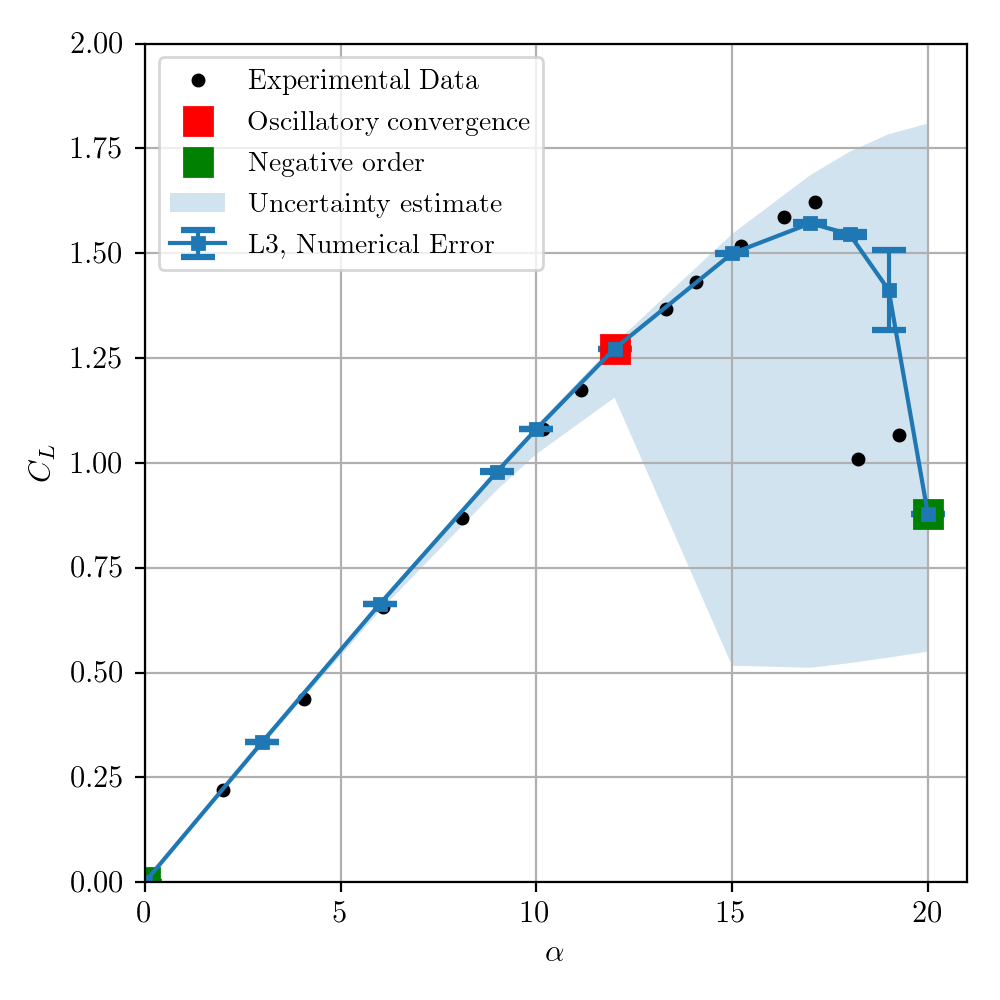
\includegraphics[width=0.6\textwidth]{code/image_gen/naca0012/images/naca0012_CL_vs_alpha_num_uq_L3.png}
\caption{Comparing the numerical discretization error bars with the turbulence modeling uncertainty areas predicted by the EQUiPS module. \label{fig:naca0012_num+turb_uq}}
\end{figure}

\subsection{ONERA M6 Wing}

A classic CFD validation case, the ONERA M6 wing is chosen as the 3D case to investigate the relationship between numerical discretization errors and turbulence modeling uncertainties. 
It is a swept, untwisted, semi-span wing that uses a symmetric airfoil, the ONERA D, as it's cross-sectional shape. 
The simulations conditions are presented in Table \ref{tab:ONERAM6_test_cond}.
A family of structured meshes is available from the NASA Turbulence Modeling Resource website.
A subset of these structured meshes are used, details for which are shown in Table \ref{tab:oneram6_meshes}.
The finest mesh level from this family, the L1 mesh, has $\ge 64$ million points. 
It would be very computationally expensive to perform the eigenspace perturbation simulations on and so it is omitted from this study.

\begin{table}
\centering
    \renewcommand{\arraystretch}{1.2}
    \captionsetup{justification=centering}
    \caption{Simulation conditions for the ONERAM6 wing.} 
    \begin{tabular}{|c|c|}
        \hline
        Mach Number & $0.84$ \\ \hline
        Reynolds Number & $14.6\times10^6$ \\ \hline
        Reference chord length & $0.805$ m \\ \hline
        Freestream Temperature & $300~\text{K}$ \\ \hline
        $\alpha$ & $3.06^\circ, 6.06^\circ$ \\ \hline 
    \end{tabular}
    \label{tab:ONERAM6_test_cond}
\end{table}

\begin{table}
    \renewcommand{\arraystretch}{1.2}
    \centering
    \begin{tabular}{ c|c|c } 
%  \hline
         Mesh Level & Nodes & Approx. $y^+$  \\ 
         \hline
         L2 & $8,677,681$ &  $1.0$\\
         L3 & $1,087,665$ &  $2.0$\\
         L4 & $136,793$ & $4.0$\\
        
    \end{tabular}
    \caption{Details of the grid family used to perform numerical discretization error quantification for the ONERA M6 case.}
    \label{tab:oneram6_meshes}
\end{table}

\begin{figure}
\center
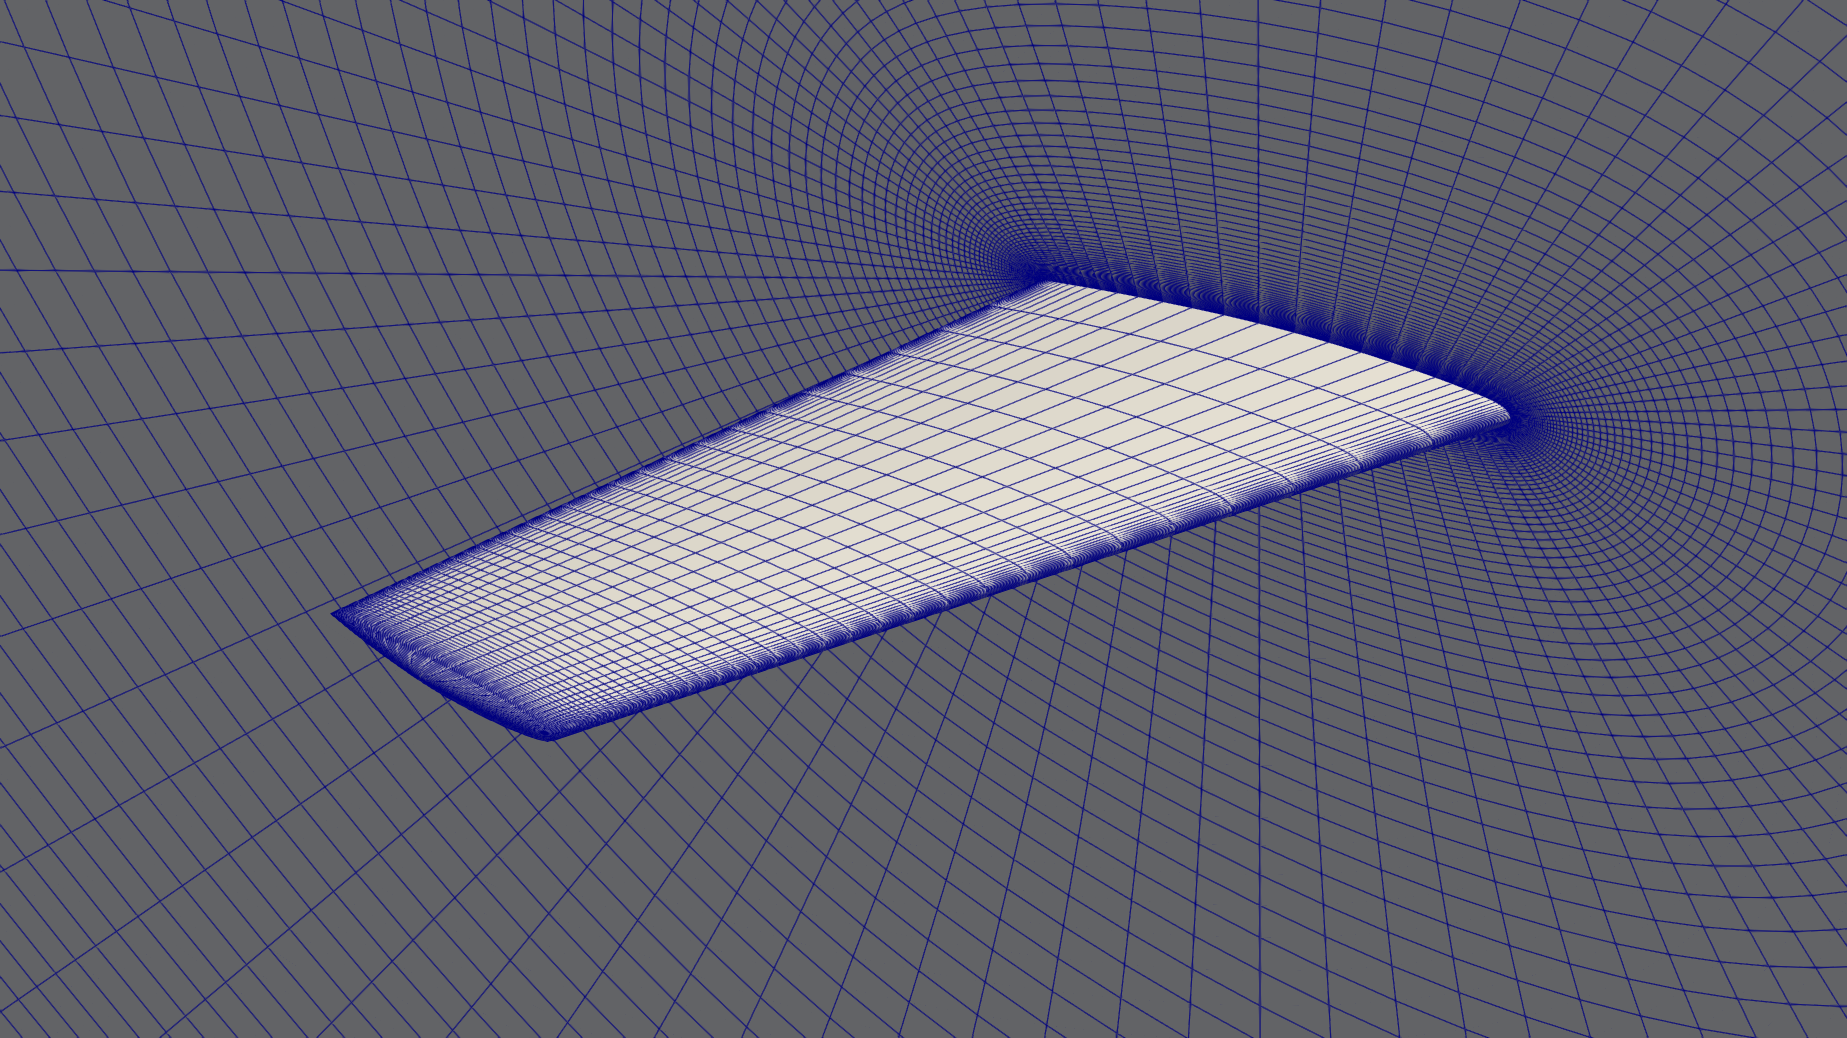
\includegraphics[width=0.6\textwidth]{code/image_gen/oneram6/images/oneram6_L3_mesh.png}
\caption{The L3 structured surface mesh for the ONERA M6. \label{fig:oneram6_mesh}}
\end{figure}

\begin{figure}
\center
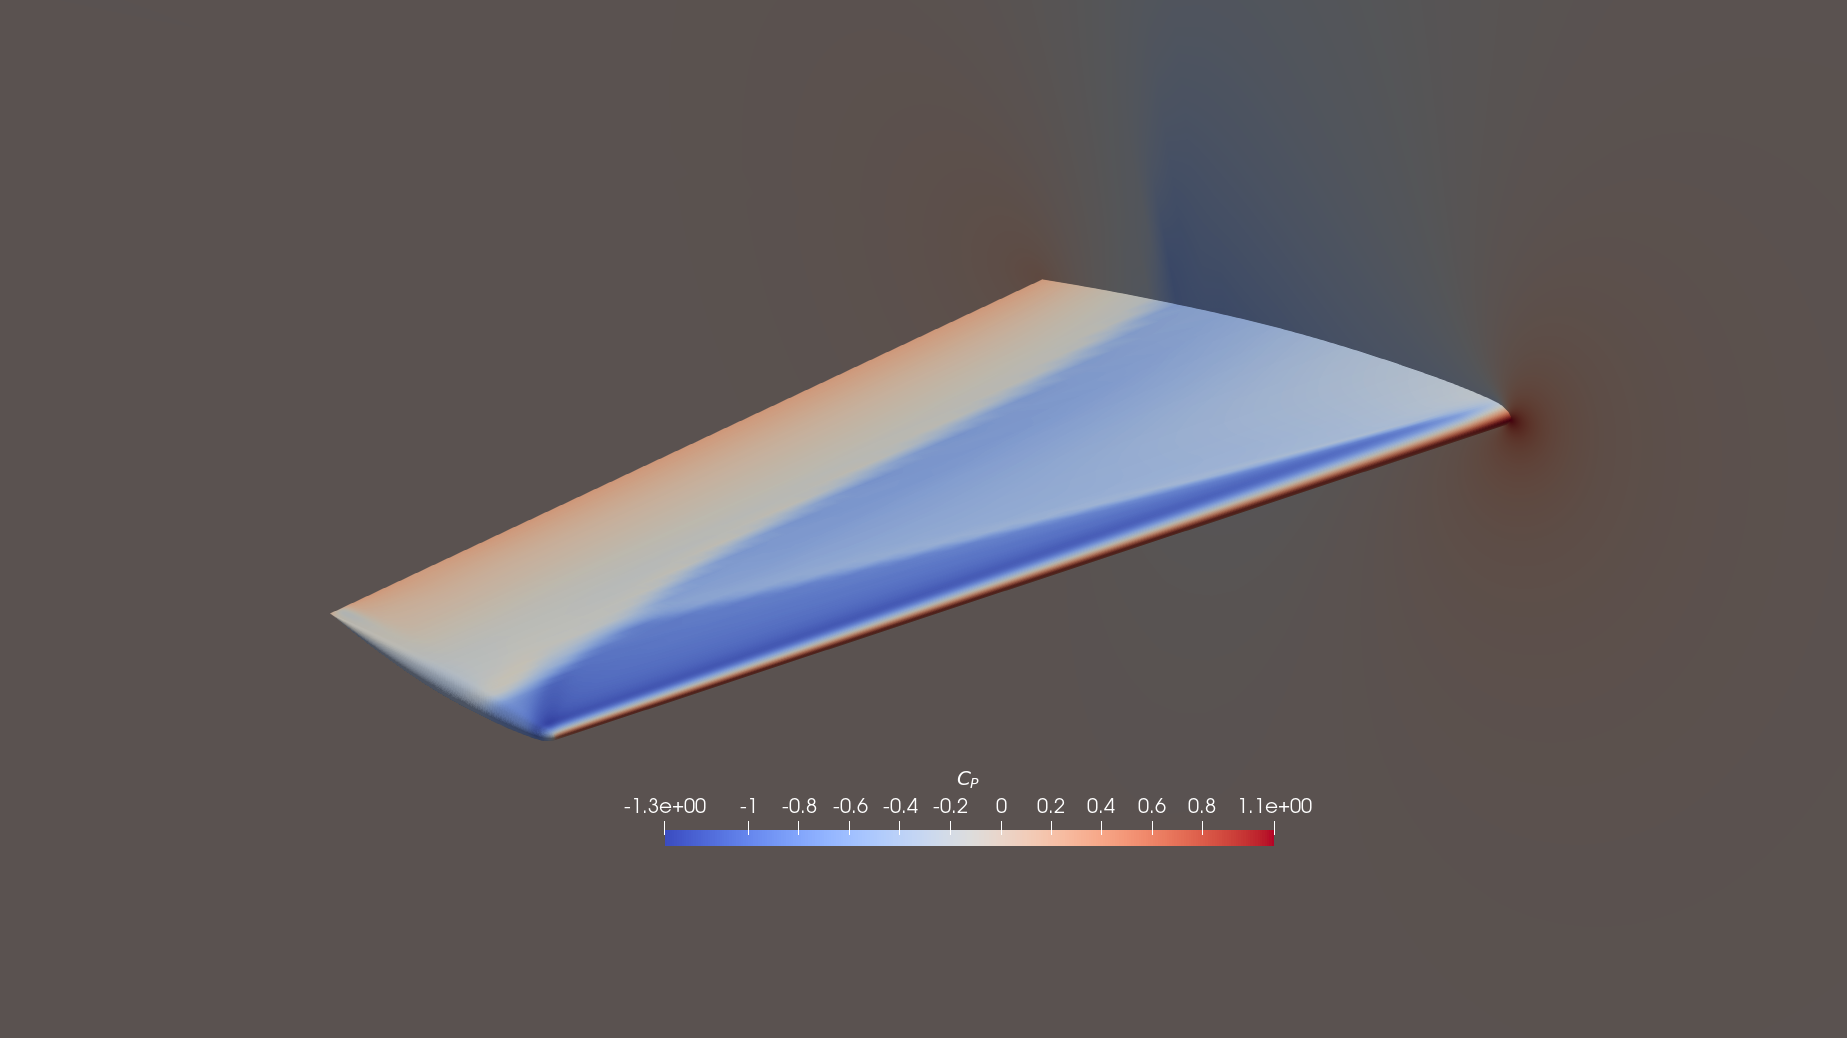
\includegraphics[width=0.6\textwidth]{code/image_gen/oneram6/images/oneram6_cp_contour.png}
\caption{Surface contour for the $C_P$ at $\alpha= 3.06^\circ$ reveals the lambda-shaped shock wave that forms on the top surface of the wing. \label{fig:oneram6_cp}}
\end{figure}

The transonic flow over the wing results in a strong $\lambda$-shock on the upper surface of the wing, as depicted in Figure \ref{fig:oneram6_cp}.
Accurate predictions for the relative locations of the two shocks and their meeting point requires sufficient mesh refinement. 
It is also a difficult feature for RANS CFD solvers to predict correctly as the turbulence model can introduce significant uncertainty in the results.
The relative magnitudes of the two estimates are compared in Figure \ref{fig:oneram6_3aoa}.
The black squares represent the baseline RANS CFD predictions and the gray shaded region represents the estimated uncertainty that is injected by the turbulence model. 
The finest mesh data point, on the left on these plots, has the numerical discretization error bars associated with it. 
Since 3 meshes are used, only the finest mesh has error metrics associated with it. 
The uncertainty estimated by the EQUiPS module is significantly larger than the errors introduced due to insufficient numerical discretization.
Additionally, the mesh refinement doesn't significantly impact the size of the uncertainty estimates. 

\begin{figure}
\center
\subfigure%[\label{subfig:oneram6_CL_3aoa} $C_L$ vs. $\alpha$ sweeps meshes of varying refinement.]
  {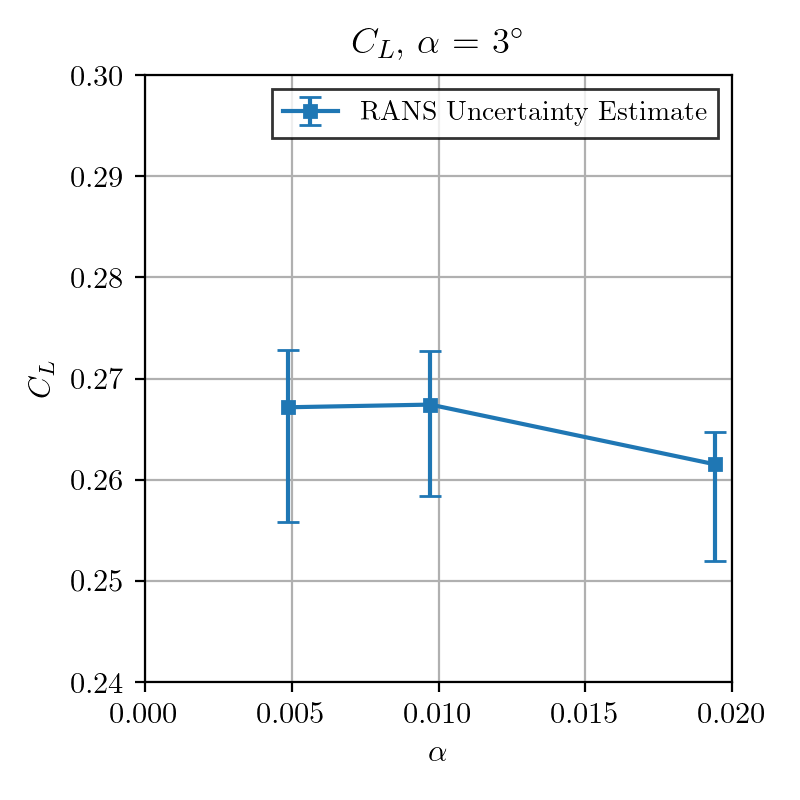
\includegraphics[width=0.48\textwidth]{code/image_gen/oneram6/images/CL_03aoa.png}}
\subfigure%[\label{subfig:oneram6_CD_3aoa} $C_D$ vs. $\alpha$ sweeps with the corresponding turbulence modeling uncertainty areas overlaid on the plot]
  {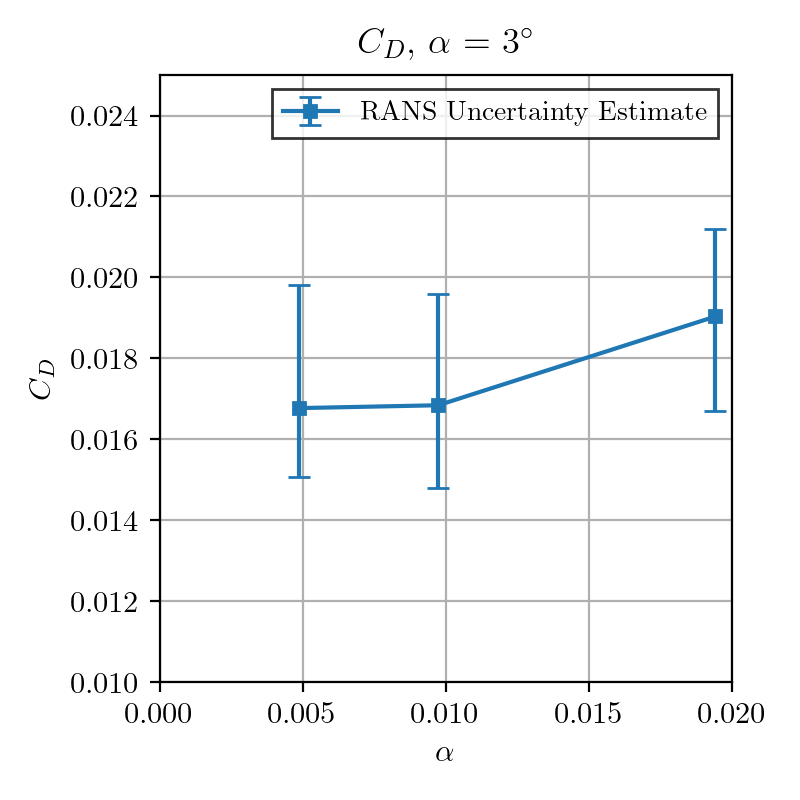
\includegraphics[width=0.48\textwidth]{code/image_gen/oneram6/images/CD_03aoa.png}}
\caption{Comparing the numerical discretization error and the turbulence modeling uncertainty estimate on $C_L$ and $C_D$ predictions at $\alpha = 3.06^\circ$ for the ONERAM6 wing.}\label{fig:oneram6_3aoa}
\end{figure}

When the angle of attack is increased to $\alpha = 6.06^\circ$, a different story unfolds. 
At such a high angle of attack, this mesh family is no longer in the asymptotic region of convergence for this case. 
This is evidenced by the oscillatory convergence characteristics seen in Figure \ref{fig:oneram6_6aoa}.
The error metrics for the discretization error are no longer valid as the grids are not sufficiently large to capture all the relevant flow physics. 
Consequently, the uncertainty estimates change drastically as the grid is refined. 

\begin{figure}
\center
\subfigure%[\label{subfig:oneram6_CL_3aoa} $C_L$ vs. $\alpha$ sweeps meshes of varying refinement.]
  {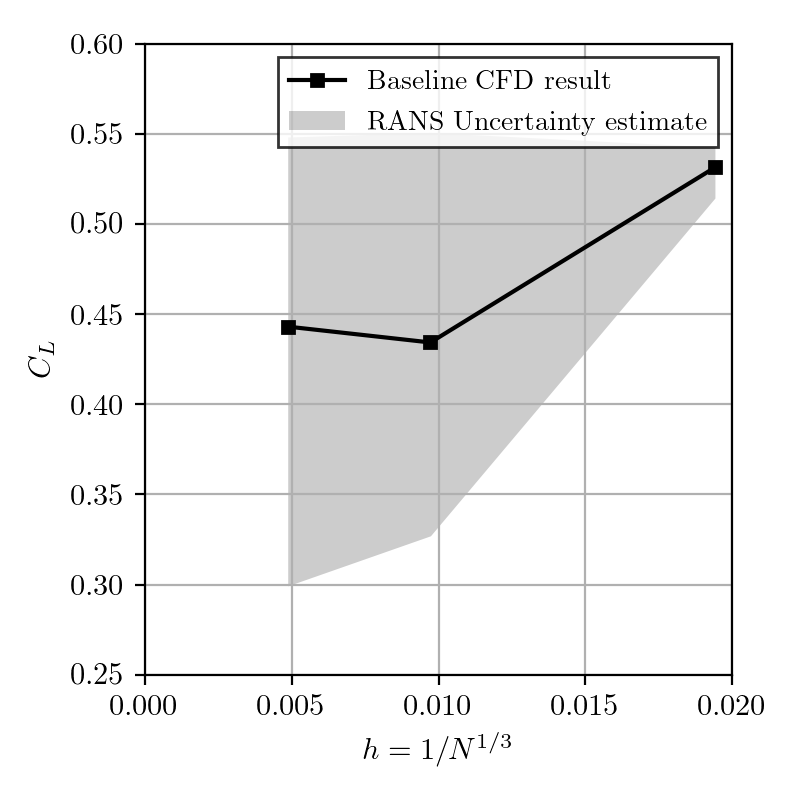
\includegraphics[width=0.48\textwidth]{code/image_gen/oneram6/images/CL_06aoa.png}}
\subfigure%[\label{subfig:oneram6_CD_3aoa} $C_D$ vs. $\alpha$ sweeps with the corresponding turbulence modeling uncertainty areas overlaid on the plot]
  {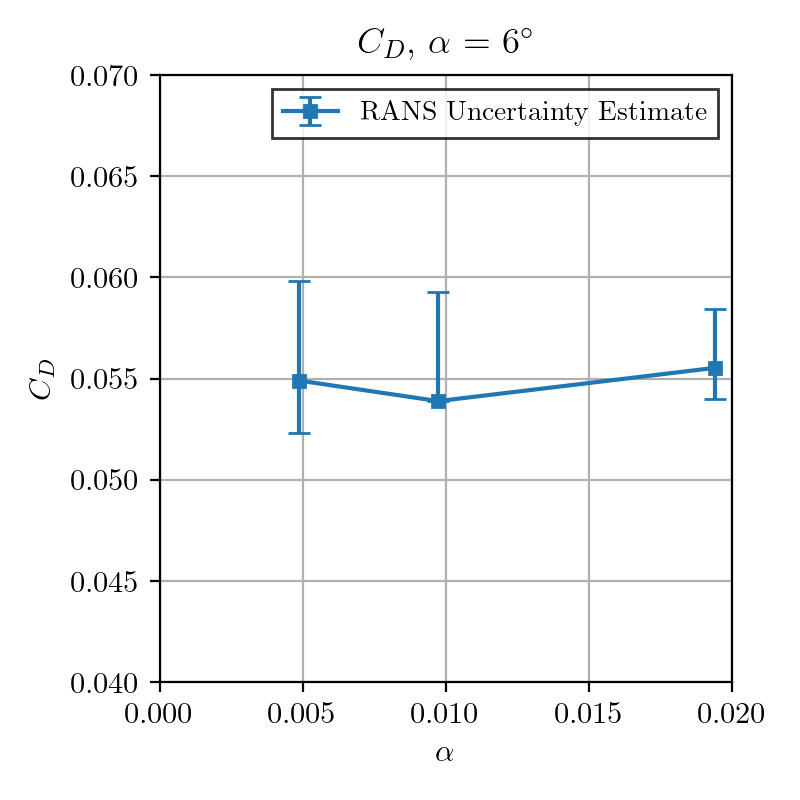
\includegraphics[width=0.48\textwidth]{code/image_gen/oneram6/images/CD_06aoa.png}}
\caption{Comparing the numerical discretization error and the turbulence modeling uncertainty estimate on $C_L$ and $C_D$ predictions at $\alpha = 6.06^\circ$ for the ONERAM6 wing.}\label{fig:oneram6_6aoa}
\end{figure}

In summary, the 2D and 3D investigations into the relationship between numerical discretization errors and the turbulence modeling uncertainty estimates yield similar results and provide guidelines for the grids that should be used with the EQUiPS module.
A minimum level of grid refinement that can capture all the relevant flow physics is required.
More specifically, the grids should be in the asymptotic region of grid convergence for the particular flow configuration in question.
This ensures that the numerical discretization error is small and that the turbulence modeling uncertainty estimate is the dominant source of error in the simulations. 
Once a grid of sufficient refinement is used, additional refinement doesn't significantly impact the turbulence modeling uncertainty estimate.
These conclusions are kept in mind when creating grids for the use with the EQUiPS module. 